\section{Implementation} 
\label{implementation}
%===============

Both the jumping mechanism and wings for deceleration will be outlined here. This section shows possible designs for the robots mechanisms.\\

%===================== Jumping Mechanism ==========
\begin{figure}[H]
\begin{center}
\subfigure[Compressed jumping mechanism]{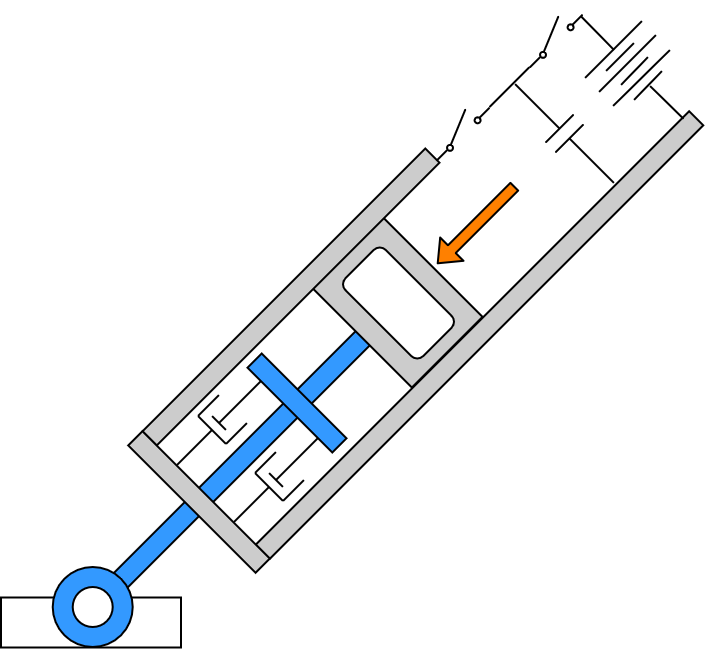
\includegraphics[width=0.4\linewidth]{./Figures/AccelerationMechanism.png} }
\subfigure[Extended jumping mechanism]{\includegraphics[width=0.4\linewidth]{./Figures/AccelerationMechanism2.png} } 
\caption{Example of a chart}
\label{fig:jumpMech}
\end{center}
\end{figure} 
%===================== Jumping Mechanism ==========

\indent The mechanical implementation for the flea-inspired jumping mechanism is shown in \textbf{Figure} \ref{fig:jumpMech}. To achieve the necessary energy density, a small battery and a large capacitor will be used. The capacitor allows for large quantities of charge to be discharged rapidly. The current will flow through the armature, pushing the piston-like leg (blue) out. The micro-controller mentioned in \textbf{section} \ref{method} will control the flow of current and capacitor charging and discharging. \\

%===================== Wings ==========
\begin{figure}[H]
\begin{center}
\subfigure[Folded wings]{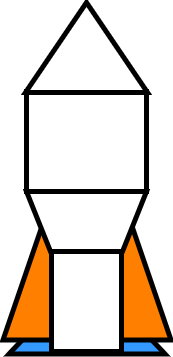
\includegraphics[height=0.3\linewidth]{./Figures/wings2.png} }
\subfigure[Extended wings]{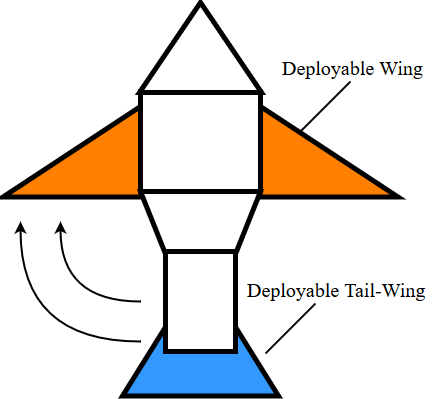
\includegraphics[width=0.4\linewidth]{./Figures/wings.png} } 
\caption{Example of a chart}
\label{fig:wings}
\end{center}
\end{figure} 
%===================== Wings ==========

\indent \textbf{Figure} \ref{fig:jumpMech} shows the deployable wings. The wings must be folded at first to maximize the height. When the wings are folded air resistance is less and the jumping mechanism can propel the robot higher. The on-board micro-controller will control the timing of the wings and when the are deployed.\\